\documentclass[11pt,a4paper]{article}

\usepackage[T1]{fontenc}
\usepackage[utf8]{inputenc}
\usepackage{amsmath,amsthm}
\usepackage{newpxtext,newpxmath}
\usepackage{fontspec}
\setmonofont[Scale=0.88]{Inconsolatazi4-Regular.otf}
\usepackage[margin=1.1in]{geometry}
\usepackage{microtype}
\usepackage{mathtools}
\usepackage{booktabs}
\usepackage{enumitem}
\usepackage{tikz}
\usepackage{xcolor}
\definecolor{linkblue}{RGB}{30,70,140}
\usepackage[colorlinks=true,linkcolor=linkblue,citecolor=linkblue,urlcolor=linkblue]{hyperref}
\usepackage[capitalise,nameinlink]{cleveref}

\setlist{itemsep=2pt,topsep=4pt}
\linespread{1.04}
\emergencystretch=2.5em

\newtheorem{theorem}{Theorem}
\renewcommand{\thetheorem}{\Alph{theorem}}
\newtheorem{thm}{Theorem}[section]
\newtheorem{lemma}[thm]{Lemma}
\newtheorem{proposition}[thm]{Proposition}
\newtheorem{corollary}[thm]{Corollary}
\theoremstyle{definition}
\newtheorem{definition}[thm]{Definition}
\theoremstyle{remark}
\newtheorem{remark}[thm]{Remark}
\crefname{thm}{Theorem}{Theorems}

\newcommand{\OO}{\mathbb{O}}
\newcommand{\ZZ}{\mathbb{Z}}
\newcommand{\RR}{\mathbb{R}}
\newcommand{\CC}{\mathbb{C}}
\newcommand{\assoc}[3]{[#1,#2,#3]}
\newcommand{\DN}{\mathrm{D}_N}
\newcommand{\ctx}{\mathcal{C}}
\newcommand{\cS}{\mathcal{S}}
\newcommand{\lean}[1]{\texttt{#1}}
\newcommand{\Bell}{\mathrm{Bell}}
\DeclareMathOperator{\rank}{rank}
\DeclareMathOperator{\ev}{ev}
\DeclareMathOperator{\supp}{supp}

\title{\vspace{-1.2em}\textbf{Flip-connectivity of octonion bracketing classes}\\[0.35em]
\large A characterization for all lengths, its Bell-number count,\\ and a Lean~4 formalization}
\author{Jes\'us Vilela Jato\\[0.2em]
\small Independent researcher, Madrid\\
\small \href{https://github.com/Dojo-1/Lemma-W-count-determinant-witness-}{\texttt{github.com/Dojo-1/Lemma-W-count-determinant-witness-}}}
\date{November 2026}

\begin{document}
\maketitle

\begin{abstract}
\noindent
Fix a word $w=w_1\cdots w_n$ in letters and substitute octonions for the letters. Each of the
$C_{n-1}$ bracketings of $w$ is a polynomial map, and bracketings inducing the same map form a
\emph{kernel class}. The bracketings are the vertices of the associahedron $K_n$, whose edges are the
flips $(AB)C\leftrightarrow A(BC)$. We prove that every kernel class of $w$ induces a connected
subgraph of $K_n$ if and only if $w$ has at most two distinct letters or every letter of $w$ occupies a
single contiguous run. Consequently, among the $\Bell(n)$ words of length $n$ up to renaming of letters,
exactly $\Bell(n)-2^n+n$ have a kernel class that is not flip-connected.

The proof has a local and a global part. Locally, a flip that preserves the map must have a
letter-count matrix of rank at most two (a count-determinant witness), and for interval words the
converse holds by Artin's theorem. Globally, for interval words the components of the graph of
rank-$\le2$ flips are separated by an explicit invariant that octonion moments detect; for non-interval
words a family of \emph{caterpillar} certificates exhibits two Moufang-equivalent bracketings in
different such components. The main theorem, the count and every lemma they use are theorems of a
Lean~4 formalization (no \texttt{sorry}, standard axioms only); the one informal step is the remark that
polynomial identities over $\ZZ^8$ and over $\RR^8$ coincide.
\end{abstract}

\noindent\textbf{MSC2020:} Primary 17D05; Secondary 17A35, 05A18, 05A15, 20N02, 05C40, 52B05, 68V20, 68V15.\\[0.2em]
\textbf{Keywords:} octonions, alternative algebras, Moufang identities, bracketings, associahedron,
flip graph, associative spectrum, Bell numbers, Lean~4, formalized mathematics.

\tableofcontents

\section{Introduction}\label{sec:intro}

In an associative algebra all bracketings of a product agree. In a nonassociative algebra they need not,
and the natural question is \emph{which} bracketings agree. For a groupoid $(G,\ast)$, Cs\'ak\'any and
Waldhauser~\cite{CW00} introduced the \emph{associative spectrum}: the number $s_n(G)$ of distinct
$n$-ary term operations induced by the bracketings of $x_1\cdots x_n$ with pairwise distinct
variables. Associative spectra have since been determined for many operations, including graph
algebras~\cite{LW22} and linear quasigroups~\cite{LW23}, and extended to $p$-ary operations~\cite{LiW09}
and to the associative--commutative setting~\cite{HL22}. The spectrum of an \emph{antiassociative}
operation is the Catalan sequence.

This paper studies a refinement in which the variables may repeat. Fix a word $w$; the bracketings of
$w$ are the vertices of the associahedron $K_n$ (Tamari~\cite{Tam62}, Stasheff~\cite{Sta63}), and two
adjacent vertices differ by one \emph{flip} $(AB)C\leftrightarrow A(BC)$ applied inside a context. Over
the octonions $\OO$, bracketings inducing the same polynomial map partition the vertex set. Repeated
letters create identities such as the Moufang laws~\cite{Mou35}, so the classes are no longer singletons,
and it becomes meaningful to ask about their \emph{shape} inside $K_n$.

\begin{definition}
A kernel class of $w$ is \emph{flip-connected} if any two of its members are joined by a path of flips
all of whose vertices lie in the class. A word is \emph{interval} if every letter occupies one
contiguous run, e.g.\ $x^ay^bz^c$.
\end{definition}

\begin{theorem}[Main theorem]\label{thm:main}
Every kernel class of bracketings of $w$ over $\OO$ is flip-connected if and only if $w$ has at most two
distinct letters or $w$ is an interval word.
\end{theorem}

\begin{theorem}[Count]\label{thm:count}
For $n\ge1$, among the $\Bell(n)$ words of length $n$ up to renaming of letters, exactly
$\Bell(n)-2^n+n$ have a kernel class that is not flip-connected. The sequence begins
$0,0,0,3,25,145,756,3892,20644,114961$ for $n=1,\dots,10$.
\end{theorem}

Both are proved below, and both are theorems of the Lean~4 formalization described in
\cref{sec:formal}: \lean{MainThm.main} and \lean{Count.count\_disconnected}. The count runs over
restricted growth strings, and \lean{Canon.canonical} shows that these contain exactly one word per
renaming class.

\paragraph{The local criterion.} Let a flip $(AB)C\to A(BC)$ act on consecutive segments $a,b,c$ of $w$,
and let $N$ be the $3\times\lvert\Lambda\rvert$ matrix of letter counts of $a,b,c$ ($\Lambda$ the
alphabet). By context cancellation (\cref{lem:L1}) the flip stays inside a kernel class exactly when the
local associator $\assoc ABC$ vanishes identically. The count-determinant witness (\cref{lem:W}) shows
that $\rank N=3$ forces $\assoc ABC\not\equiv0$. We write $\DN$ for the set of flips whose count matrix is
degenerate ($\rank N\le2$) and call them \emph{$\DN$-flips}. So in-class flips are $\DN$-flips, and two
equal maps in different components of the $\DN$-flip graph certify a disconnected class. The converse
fails in general (in $xyzyx$ the flip on $xy\,|\,z\,|\,yx$ has $\rank N=2$ and a nonzero associator), but
it holds for interval words (\cref{lem:V,lem:I}).

\paragraph{Interval words (Theorem~G2, \cref{thm:G2}).} We classify the $\DN$-components of an interval
word by the shapes that a bracketing induces on leaf triples with three distinct letters
(\cref{prop:C}), reduce separation to three-block words $x^ay^bz^c$, and describe their components by an
explicit invariant (\cref{prop:T}). Substituting $x=1+se_1$, $y=1+qe_2$, $z=1+te_4$ turns every
bracketing into a polynomial whose $s^pqt^r$ coefficients are \emph{moments} of the invariant
(\cref{lem:M}); these moments determine the invariant (\cref{prop:S}). Hence distinct components are
distinct maps.

\paragraph{Non-interval words (Theorem~G3, \cref{thm:G3}).} For a three-letter non-interval word we build
a bracketing $T_0$ along a \emph{caterpillar}, a sequence of peels of end runs, and a Moufang move
$T_0\to T_1$ deleting one of its nodes (\cref{fig:moufang}). The caterpillar's nodes form a
\emph{self-certifying} set: every rotation that would delete one of them has a rank-$3$ count matrix
(\cref{lem:Cat}), so no $\DN$-path from $T_0$ can lose them (\cref{lem:Rprime}). An induction on run
sequences shows that every non-interval three-letter word has such a caterpillar (\cref{prop:E}).
Specialising extra letters to $1$ lifts the result to words with more letters (\cref{lem:K}).

\paragraph{Formalization.} The development is a Lean~4~\cite{Lean} project of 9{,}252 lines in 30 files
using only the core library. Octonion identities are proved by a verified polynomial normaliser, the
finite base of the run-sequence induction by kernel evaluation, and everything else by ordinary proofs.
The theorems of \cref{tab:lean} depend only on \texttt{propext}, \texttt{Classical.choice} and
\texttt{Quot.sound} (log in the repository). A second implementation in Prolog runs the constructions and
checks their outputs on small words (\cref{sec:checks}).

\paragraph{Scope of valuations.} ``Equal maps'' means equal as polynomial maps, equivalently equal on
all real octonions. The formal development quantifies over \emph{integer} octonions $\ZZ^8$. Every
bracketing is a polynomial with integer coefficients in the $8\lvert\Lambda\rvert$ coordinates, and a
polynomial vanishing on $\ZZ^{8\lvert\Lambda\rvert}$ is zero, so the notions coincide; this is the only step
outside the formal proof.

\section{Preliminaries}\label{sec:prelim}

\subsection{Octonions}
Let $\OO$ be the real algebra with basis $e_0=1,e_1,\dots,e_7$ and product
$e_ie_j=\varepsilon(i,j)\,e_{i\oplus j}$, where $\oplus$ is bitwise exclusive or and
$\varepsilon(i,j)\in\{\pm1\}$ is a Cayley--Dickson sign table~\cite{Bae02} with $e_i^2=-1$ for $i\ge1$.
$\OO$ is an alternative division algebra; its norm form $\nu(x)=x\bar x$ is multiplicative. We write
$\assoc abc=(ab)c-a(bc)$; the associator is trilinear and alternating, and vanishes when one argument is
real. We use:
\begin{itemize}
  \item the Moufang identities~\cite{Mou35} $a(b(ac))=((ab)a)c$, $((ca)b)a=c(a(ba))$,
    $(ab)(ca)=a((bc)a)$;
  \item Artin's theorem: the subalgebra generated by any two elements is associative~\cite{Sch66,ZSSS82};
  \item for $X,Y,Z\in\operatorname{span}(e_1,e_2,e_4)$ with coordinate vectors $x,y,z\in\RR^3$,
    $\assoc XYZ=2\det(x,y,z)\,e_7$; in particular $\assoc{e_1}{e_2}{e_4}=2e_7$.
\end{itemize}
All three are polynomial identities with integer coefficients; in the formalization they are proved for
$\ZZ^8$ by a normaliser.

\subsection{Words, bracketings, flips}
A word $w=w_1\cdots w_n$ is a finite sequence over an alphabet $\Lambda$. A \emph{bracketing} is a
planar binary tree $T$ with leaves $1,\dots,n$ in order. For a valuation $\rho\colon\Lambda\to\OO$,
$\ev_T(\rho)$ is the product of $\rho(w_1),\dots,\rho(w_n)$ bracketed by $T$, and $T\sim T'$ if
$\ev_T=\ev_{T'}$ for all $\rho$. A subtree spans a \emph{segment}, a set of consecutive positions. A
\emph{context} $\ctx[\,\cdot\,]$ is a tree with one hole. A \emph{flip} replaces $\ctx[(AB)C]$ by
$\ctx[A(BC)]$ or back; bracketings and flips form the associahedron $K_n$.

For a flip on segments $a,b,c$ let $N\in\ZZ^{3\times\lvert\Lambda\rvert}$ be the matrix of letter counts.
The flip is a \emph{$\DN$-flip} if $\rank N\le2$. Since $N$ depends only on the segments, this does not
depend on $A,B,C$ or on the context.

\subsection{Run sequences}
Collapsing maximal runs of equal letters gives the \emph{run sequence} of $w$; $w$ is interval iff its
run sequence has no repeated letter. A word with at least three letters that is not interval contains a
pattern $p\cdots q\cdots p$ with $q\ne p$; with any third letter $r$, its restriction to $\{p,q,r\}$ is
again non-interval.

\section{Local lemmas}\label{sec:local}

\begin{lemma}[context cancellation, L1]\label{lem:L1}
For every context $\ctx$ and bracketings $S_1,S_2$ of the same segment, $\ctx[S_1]\sim\ctx[S_2]$ iff
$S_1\sim S_2$. Consequently a flip $\ctx[(AB)C]\to\ctx[A(BC)]$ stays inside a kernel class iff
$\assoc ABC\equiv0$.
\end{lemma}
\begin{proof}
$\ctx[S]$ is $S$ composed with left and right multiplications by values of the other subtrees of
$\ctx$. If all letter values are nonzero these values are nonzero, and multiplication by a nonzero
octonion is injective since $\nu$ is multiplicative. So $\ctx[S_1]=\ctx[S_2]$ at a valuation with
nonzero letters forces $S_1=S_2$ there; such valuations are Zariski dense. The converse is clear.
\end{proof}

\begin{lemma}[count-determinant witness, W]\label{lem:W}
If $\rank N=3$, then $\assoc ABC\not\equiv0$ for all bracketings $A,B,C$ of $a,b,c$. Precisely, if the
minor of $N$ on letters $x,y,z$ is $d\ne0$ and $M=2\lvert d\rvert+1$, the integer valuation
$x\mapsto1+Me_1$, $y\mapsto1+Me_2$, $z\mapsto1+Me_4$, other letters $\mapsto1$, gives
\[
  \assoc ABC\equiv 2dM^3e_7 \pmod{M^4\ZZ^8},
\]
which is nonzero. All letter values have real part $1$.
\end{lemma}
\begin{proof}
Write the letter values as $1+Mq_\ell$ with $q_x=e_1$, $q_y=e_2$, $q_z=e_4$, $q_\ell=0$ otherwise.
Products respect congruences mod $M^4$, so a bracketing $S$ of a segment $s$ satisfies
$\ev_S\equiv1+M\Sigma_s+M^2P_2+M^3P_3$, the product of truncated power series, where
$\Sigma_s=\sum_\ell N_{s\ell}q_\ell$ depends only on the counts. In the associator of three such
elements the terms of order $M^0,M^1,M^2$ cancel because the associator vanishes when an argument is
real, and the term of order $M^3$ is $\assoc{\Sigma_a}{\Sigma_b}{\Sigma_c}=2de_7$. If $\assoc ABC=0$
then $M^4\mid2dM^3$, so $M\mid2d$, contradicting $0<\lvert2d\rvert<M$. (Over $\RR$,
$x\mapsto\exp(\theta e_1)$ etc.\ gives $\assoc ABC=2d\theta^3e_7+O(\theta^4)$.)
\end{proof}

\begin{corollary}\label{cor:Wflip}
For every word, every flip that stays inside a kernel class is a $\DN$-flip. Hence two equal maps in
different components of the $\DN$-flip graph lie in a kernel class that is not flip-connected.
\end{corollary}
\begin{proof}
\Cref{lem:L1,lem:W}; the witness valuation has nonzero letter values, as context cancellation requires.
\end{proof}

\begin{lemma}[vanishing, V]\label{lem:V}
$\assoc ABC\equiv0$ if the segments $a,b,c$ together use at most two letters, or if two of $a,b,c$ are
powers of the same letter.
\end{lemma}
\begin{proof}
In the first case all three values lie in the subalgebra generated by two letter values. In the second,
two values lie in $\operatorname{span}\{1,x\}$ ($\OO$ is quadratic), so all three lie in the subalgebra
generated by $x$ and the third value. Artin's theorem makes either subalgebra associative.
\end{proof}

\begin{lemma}[interval rank, I]\label{lem:I}
Let $w$ be interval and $a,b,c$ consecutive segments using at least three letters, such that no two of
$a,b,c$ are powers of the same letter. Then $\rank N=3$.
\end{lemma}
\begin{proof}
Order the letters by block, so that $\max\supp(a)\le\min\supp(b)$ and $\max\supp(b)\le\min\supp(c)$.

\emph{Case $\supp(b)=\{p\}$.} Neither $a$ nor $c$ is a power of $p$, so $a$ has a letter $x<p$ and $c$ a
letter $z>p$. On columns $(x,p,z)$,
\[
  N_{xpz}=\begin{pmatrix}a_x&a_p&0\\0&b_p&0\\0&c_p&c_z\end{pmatrix},\qquad \det N_{xpz}=a_xb_pc_z\ne0.
\]

\emph{Case $\lvert\supp(b)\rvert\ge2$}, with $p=\min\supp(b)<q=\max\supp(b)$; then
$\supp(a)\cap\supp(c)=\emptyset$. Either $\supp(a)=\{p\}$ or $a$ has a letter $x<p$; either
$\supp(c)=\{q\}$ or $c$ has a letter $z>q$; let $y\in\supp(b)$ with $p<y<q$ when it exists. Take the first
column $x$ (or $p$), the last column $z$ (or $q$), and the middle column $y$, or, if no such $y$ exists,
the letter of $\{p,q\}$ not already used. Row $a$ vanishes outside the first column and the column $p$;
row $c$ vanishes outside the last column and the column $q$. In every combination one of these rows has a
single nonzero entry; expanding along it leaves a triangular $2\times2$ block, so the determinant is a
product of three nonzero counts. For instance, if $\supp(a)=\{p\}$ and $\supp(c)=\{q\}$ ($y$ then exists
by the three-letter hypothesis), on columns $(p,y,q)$ the matrix is
\[
  \begin{pmatrix}a_p&0&0\\b_p&b_y&b_q\\0&0&c_q\end{pmatrix},
\]
not triangular, with determinant $a_pb_yc_q\ne0$.
\end{proof}

\Cref{lem:V,lem:I} together say that in an interval word every $\DN$-flip has a vanishing associator.

\begin{lemma}[killing, K]\label{lem:K}
Setting a set of letters to $1$ sends bracketings of $w$ to bracketings of the subword $w'$ (or to the
empty product). It maps $\DN$-flips to $\DN$-flips or to identities, and equal maps to equal maps.
Moufang moves whose repeated variable is a single letter \emph{lift}: if $T_0'\to T_1'$ is such a move
of $w'$ joining different $\DN$-components of $w'$, there is such a move $T_0\to T_1$ of $w$ restricting
to it and joining different $\DN$-components of $w$.
\end{lemma}
\begin{proof}
Deleting columns of $N$ cannot raise its rank, and specialisation preserves identities. In the patterns
$x(Y(xC))$, $((Cx)Y)x$ and $x((BC)x)$ every gap between consecutive surviving leaves borders a
non-repeated variable ($Y$, $B$ or $C$) or the context, so the killed leaves can be absorbed there, and
the lifted move is again such a Moufang move. A $\DN$-path between the lifts would restrict to a
$\DN$-path, or a constant path, between $T_0'$ and $T_1'$.
\end{proof}

\section{Interval words: Theorem G2}\label{sec:interval}

\subsection{Components and triple shapes}

\begin{proposition}[Proposition C]\label{prop:C}
Let $w$ be interval. For a bracketing $T$ let $\tau(T)$ record, for every leaf triple $i_1<i_2<i_3$ with
pairwise distinct letters, whether $T$ induces $((i_1i_2)i_3)$ or $(i_1(i_2i_3))$. Then $T,T'$ lie in the
same $\DN$-component iff $\tau(T)=\tau(T')$.
\end{proposition}
\begin{proof}
($\Rightarrow$) A flip $(AB)C\to A(BC)$ changes exactly the shapes of the triples in $A\times B\times C$.
If it is a $\DN$-flip, by \cref{lem:I} $abc$ has at most two letters or two of $a,b,c$ are powers of the
same letter; in an interval word, if $a$ and $c$ are powers of $x$ then so is $b$. In every case each
triple of $A\times B\times C$ repeats a letter, so $\tau$ is unchanged.

($\Leftarrow$) Induction on $n$; words with at most two letters have a single component. Let
$T=(T_L,T_R)$ and $T'=(T'_L,T'_R)$ have root splits after positions $m$ and $m'$. If $m=m'$, $\tau$
restricts to both factors and $\DN$-flips inside a subtree are $\DN$-flips of $T$; induction applies.
Say $m<m'$. Every triple in $[1,m]\times(m,m']\times(m',n]$ has shape $i_1(i_2i_3)$ in $T$ and
$(i_1i_2)i_3$ in $T'$, so no such triple has three distinct letters. With letter sets $X,Y,Z$ of the
three segments, ordered by block, every $x\in X,y\in Y,z\in Z$ has $x=y$ or $y=z$. If
$\lvert Y\rvert\ge3$ a middle letter gives a distinct triple; if $Y=\{y_1<y_2\}$ then $X=\{y_1\}$,
$Z=\{y_2\}$ and $w$ has two letters. So $Y=\{y\}$ and $X=\{y\}$ or $Z=\{y\}$. If $X=Y=\{y\}$, let
$T''=(P,T'_R)$ on $w[m+1..n]$ with any bracketing $P$ of $(m,m']$; its distinct-letter triples lie in
$(m',n]$ or have shape $i_1(i_2i_3)$ with $i_1\in(m,m']$, where $T$ agrees with $T'$. So
$\tau(T_R)=\tau(T'')$, and by induction $T_R$ and $T''$ are $\DN$-connected. The flip
$(T_L,(P,T'_R))\to((T_L,P),T'_R)$ is a $\DN$-flip ($a,b$ are powers of $y$) producing root split $m'$,
which reduces to the case $m=m'$. The case $Y=Z=\{y\}$ is symmetric.
\end{proof}

\subsection{Three-block words}

Let $w=x^ay^bz^c$ with $a,b,c\ge1$. For a bracketing $T$, the \emph{core} $\kappa=(U,V)$ is the lowest
node containing the last $x$ and the first $z$. Then $U=x^{a'}y^j$ and $V=y^{b-j}z^{c'}$ with
$a',c'\ge1$, and every proper ancestor of $\kappa$ attaches a pure-$x$ block on the left or a pure-$z$
block on the right. Let $W$ be the word in $\{x,z\}$ of attached letters read from $\kappa$ outward, and
$\Phi(T)=(j,a',c',W)$.

\begin{proposition}[Proposition T]\label{prop:T}
On the $\DN$-components of $x^ay^bz^c$: $j$ is invariant; for $0<j<b$, $\Phi$ is a complete invariant;
for $j=0$ (resp.\ $j=b$) the complete invariant is the join word from the core outward in which the core
$x$'s (resp.\ $z$'s) merge with the adjacent outer run.
\end{proposition}
\begin{proof}
By \cref{prop:C}, components are the fibres of $\tau$. For a three-block word, $\tau(T)$ is determined
by, and determines, the function assigning to each pair $(y_k,z_l)$ the number of $x$'s grouped with
$y_k$ before $z_l$; translating this function into $\Phi$ (respectively the join word) gives the stated
invariants. The bookkeeping is routine but long, and we rely on its formal version
(\lean{PropT.propT}: same $\DN$-component $\iff$ same invariant, via \lean{propC\_iff},
\lean{sig\_iff\_cx} and \lean{key\_iff\_cx}). For orientation, the rotations that change $\Phi$ have
determinants $\pm\,i\,j\,c'$ (an $x$-block of size $i$ crossing the core, including splitting $U$),
$\pm\,a'(b-j)k$ (the mirror, with a $z$-block of size $k$), $\pm\,a'k\,c'$ (moving $k$ letters $y$ across
$\kappa$) and $\pm\,i\,k\,n_y$ (an $x$-attachment against a $z$-attachment through a node containing
$n_y\ge1$ letters $y$); merging adjacent attachments on one side is a $\DN$-flip leaving $W$ unchanged.
Hence $j$ never changes, and for interior $j$ neither do $a',c'$; for $j=0$ only the core $x$'s can merge
outward, and symmetrically for $j=b$.
\end{proof}

\begin{remark}
Counting the realisable invariants gives
$(b-1)\bigl(\binom{a+c}{a}-1\bigr)+\binom{a+c-1}{a}+\binom{a+c-1}{c}=1+b\bigl(\binom{a+c}{a}-1\bigr)$
components, using $\sum_{i<a,\,k<c}\binom{i+k}{i}=\binom{a+c}{a}-1$. This count is not used in the proof
of \cref{thm:main}. The binomial identity is formal (\lean{Octonion.propT\_count}); the count of
components itself is verified exhaustively for small $a,b,c$ (\cref{sec:checks}) but not formalized.
\end{remark}

\subsection{Moments}

Substitute $x=1+se_1$, $y=1+qe_2$, $z=1+te_4$ and let $\mu_T(p,r)\in\OO$ be the coefficient of
$s^pqt^r$ in $\ev_T$. For a word $\omega$ in $\{x,z\}$ let $P_\omega$ be the ordered product of $1+sX$
per $x$ and $1+tZ$ per $z$ in the Clifford algebra with $X^2=Z^2=1$, $XZ=-ZX$, and write
$P_\omega=\sum_{p,r}\Gamma_\omega(p,r)\,s^pt^r\,X^{[p]}Z^{[r]}$ with $\Gamma_\omega(p,r)\in\ZZ$ and
$[p]=p\bmod2$. Put $\omega_+=x^{a'}z^{c'}W$ and $\omega_-=z^{c'}x^{a'}W$.

\begin{lemma}[moment formula, M]\label{lem:M}
There are signs $\varepsilon_{p,r}$ and signed units $E_{p,r}=\pm e_1^{[p]}e_4^{[r]}e_2$, independent
of $T$, with
\[
  \mu_T(p,r)=\varepsilon_{p,r}\bigl[\,j\,\Gamma_{\omega_+}(p,r)+(b-j)\,\Gamma_{\omega_-}(p,r)\bigr]E_{p,r}.
\]
\end{lemma}
\begin{proof}
$\mu_T(p,r)$ sums, over choices of $p$ leaves $x$, one leaf $y_k$ and $r$ leaves $z$, the value of $T$
with the chosen leaves set to $e_1,e_2,e_4$ and the others to $1$. Let
$H=\langle e_1,e_4\rangle\cong\mathbb H$ and $\ell=e_2\perp H$, so $\OO=H\oplus H\ell$ with
$h(c\ell)=(ch)\ell$ and $(c\ell)h=(c\bar h)\ell$. Subtrees without $y_k$ take values in the associative
$H$. Walking from $y_k$ to the root, the value keeps the form $c\ell$: a left sibling $h$ appends $h$, a
right sibling appends $\bar h$. After setting unchosen leaves to $1$, right siblings contain only $z$'s,
and $\overline{e_4^m}=(-1)^me_4^m$. So the value is $(-1)^re^{\omega_k}\ell$, where $\omega_k$ is the
word of absorbed blocks read bottom-up. By the definition of the core, the ancestors of $y_k$ absorb the
core and then the attachments in the order $W$; if $y_k$ lies in the core's left child ($j$ choices) the
core is absorbed as $x^{a'}z^{c'}$, otherwise as $z^{c'}x^{a'}$. Summing over subsets and reordering to
$e_1^{[p]}e_4^{[r]}$, with signs that depend only on $(p,r)$, gives the formula; the Clifford relations
match those of $e_1,e_4$ up to these signs.
\end{proof}

\begin{proposition}[separation, S]\label{prop:S}
Distinct $\DN$-components of $x^ay^bz^c$ have distinct maps; already the moments $\mu(p,1)$ and
$\mu(1,r)$ separate them.
\end{proposition}
\begin{proof}
In the $t$-linear part of $P_\omega$, a $z$ preceded by $\alpha$ letters $x$ contributes
$u^\alpha Zu^{a-\alpha}=Z\bar u^\alpha u^{a-\alpha}$ with $u=1+sX$, $\bar u=1-sX$; on the eigenline
$X=+1$ these are $(1-s)^\alpha(1+s)^{a-\alpha}$, $\alpha=0,\dots,a$, a basis of polynomials of degree
$\le a$. So the $t$-linear moments determine the weighted profile
$\zeta(\alpha)=j\,\zeta_{\omega_+}(\alpha)+(b-j)\,\zeta_{\omega_-}(\alpha)$, where $\zeta_\omega(\alpha)$
counts the $z$'s of $\omega$ preceded by exactly $\alpha$ letters $x$; symmetrically the $s$-linear
moments determine the $x$-profile $\xi$. Explicitly
\[
  \zeta=b\,\zeta_W(\cdot-a')+jc'\delta_{a'}+(b-j)c'\delta_0,\qquad
  \xi=b\,\xi_W(\cdot-c')+ja'\delta_0+(b-j)a'\delta_{c'}.
\]
Since $b\ge1$, $\zeta(0)$ and $\xi(0)$ are not both $0$. If both are positive, $j$ is interior,
$a'=\min\{\alpha>0:\zeta(\alpha)\ne0\}$, $c'=\min\{\gamma>0:\xi(\gamma)\ne0\}$, $j=b-\zeta(0)/c'$, and
$\zeta_W$ follows; a binary word is determined by its $z$-profile and its number of $x$'s, so $W$ is
determined. If $\xi(0)=0$ then $j=0$ and $\zeta=b\,\zeta_{\omega_-}$; if $\zeta(0)=0$ then $j=b$ and
$\zeta=b\,\zeta_{\omega_+}$; either way the profile determines the join word, the complete invariant for
boundary $j$ (\cref{prop:T}).
\end{proof}

In the formalization all moments are read off a single integer valuation: the coefficient of $s^pqt^r$
is recovered from one Kronecker point $s=\beta$, $q=\beta^{a+b+c+1}$, $t=\beta^{(a+b+c+1)^2}$ with
$\beta=2^{a+b+c+2}+1$, using an explicit bound on all coefficients (\lean{Coeff.coef\_of\_map}).

\subsection{Theorem G2}

\begin{thm}[G2]\label{thm:G2}
In an interval word, two bracketings are equal maps iff they lie in the same $\DN$-component. Every
kernel class is a $\DN$-component and is flip-connected.
\end{thm}
\begin{proof}
If $T,T'$ lie in different components, by \cref{prop:C} they differ on a triple with letters $p<q<r$.
Kill every other letter (\cref{lem:K}); both restrictions are bracketings of $p^aq^br^c$ that still
differ on that triple, hence lie in different components (\cref{prop:C}), hence are different maps
(\cref{prop:S}); killing is a specialisation, so $T\not\sim T'$. Conversely, by \cref{lem:I} every
$\DN$-flip of an interval word uses at most two letters or has two segments that are powers of the same
letter, so by \cref{lem:V} its associator vanishes and it stays in the class.
\end{proof}

\begin{corollary}\label{cor:distinct}
If all letters of $w$ are distinct, the $C_{n-1}$ bracketings are pairwise distinct maps, so the
associative spectrum of $\OO$ is the Catalan sequence.
\end{corollary}
\begin{proof}
This follows from \cref{thm:G2}, but directly: distinct planar binary trees induce different shapes on
some leaf triple; kill every other letter, and $\assoc xyz\not\equiv0$.
\end{proof}
The direct proof uses only a two-sided identity (to kill letters) and one non-associative triple, so it
shows $s_n(G)=C_{n-1}$ for every non-associative magma $G$ with a two-sided identity. We have not found
this stated explicitly in the associative-spectrum literature (Huang and Lehtonen~\cite{HL22} treat
related questions for groupoids with a neutral element), but given its two-line proof we expect it to be
known.

\section{Non-interval words: Theorem G3}\label{sec:noninterval}

Throughout this section $w$ uses exactly three letters and is not interval. Write $[i,i']$ for
intervals of positions and identify a bracketing with its set of internal nodes.

\subsection{Stable nodes}

\begin{lemma}[self-certifying sets, R$'$]\label{lem:Rprime}
Let $T$ be a bracketing and $\cS$ a set of nodes of $T$ such that every rotation that would delete some
$J\in\cS$ has a rank-$3$ count matrix; here a rotation deleting $J$ has children $J_1,J_2$ of $J$ and a
sibling $I$, with $J_1,J_2,I,J\cup I$ laminar with $\cS$ and the created node laminar with
$\cS\setminus\{J\}$. Then every bracketing in the $\DN$-component of $T$ contains $\cS$.
\end{lemma}
\begin{proof}
On a $\DN$-path from $T$ take the first bracketing that loses some $J\in\cS$. Its predecessor contains
$\cS$, so the deleting rotation satisfies the laminarity conditions, has rank $3$, and is not a
$\DN$-flip.
\end{proof}

\subsection{Caterpillars}

Let the run sequence of $w$ be $s_0\cdots s_{R-1}$. A \emph{caterpillar} is a sequence of steps peeling
runs off the ends of the current interval of runs: \textbf{L} peels the left run, \textbf{R} the right
run, and \textbf{D} both end runs when they carry the same letter; it stops at a \emph{bottom} of two
runs. Its intervals $J_0=w\supset J_1\supset\cdots\supset J_h$ give $\cS=\{J_1,\dots,J_h\}$. The
bracketing $T_0$ has every $J_k$ as a node; peeled runs hang off the path letter by letter, except where
a move below needs a peeled run as a single subtree (the block $Y$ of M-left, and the pattern $x((BC)x)$
of M-mid).

\begin{lemma}[Lemma Cat]\label{lem:Cat}
$\cS$ is self-certifying for $T_0$ provided
\begin{description}[font=\normalfont\itshape]
  \item[(C1)] every $J_k$ with $1\le k<h$, entered by peeling letter $\alpha$ and left by peeling letter
    $\beta$, has $\alpha\ne\beta$, and the third letter $\gamma(\alpha,\beta)$ occurs in $J_{k+1}$;
  \item[(C2)] the bottom $J_h$, with runs $u,v$ and entry letter $\alpha$, has $\alpha,u,v$ pairwise
    distinct.
\end{description}
\end{lemma}
\begin{proof}
Let $J\in\cS$ and consider a rotation deleting $J$. Laminarity with the nearest $\cS$-ancestor forces
the sibling to be a piece $\alpha^i$ of the run(s) peeled to reach $J$; laminarity with the next node
$J'\in\cS$ forces the split of $J$ to cut inside a run peeled next, a piece $\beta^{i'}$, with $J'$ whole
on the other side (at the bottom any split is allowed). So two segments are single-letter pieces and
$\det N=\pm\,i\,i'\cdot(\text{count of }\gamma(\alpha,\beta)\text{ in the third segment})\ne0$, the
third segment containing $J'$. At the bottom a direct $3\times3$ computation gives
$\pm i\cdot(\cdots)\cdot\det(e_\alpha,e_u,e_v)\ne0$.
\end{proof}

A Moufang move whose repeated variable is a single letter and which deletes a node of $\cS$ then joins
two different $\DN$-components (\cref{fig:moufang}). Three moves arise:
\begin{itemize}
  \item \textbf{M-mid.} A \textbf{D} step at $J_k=x^m\,BC\,x^{m'}$, where $T_0$ contains $x((BC)x)$ with
    $BC=J_{k+1}$: the move $x((BC)x)\to(xB)(Cx)$ deletes $J_{k+1}$.
  \item \textbf{M-left.} Two consecutive \textbf{L} steps peeling runs $u$ and $Y$, where the next left
    run carries the letter of $u$ and the following step is \textbf{L} or the bottom: with $Y$ a single
    subtree, $x(Y(xC))\to((xY)x)C$ deletes $J_{k+1}$.
  \item \textbf{M-right.} The mirror image of M-left.
\end{itemize}

\begin{figure}[t]
\centering
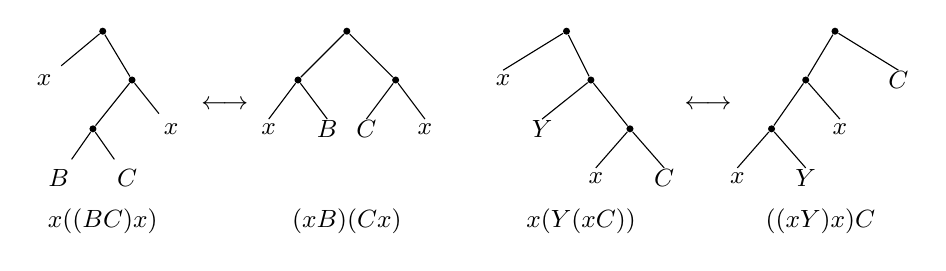
\begin{tikzpicture}[scale=0.62,every node/.style={font=\small},
  nd/.style={circle,fill=black,inner sep=0.9pt}]
\begin{scope}
  \node[nd] (r) at (0,0) {};
  \node (x) at (-1.2,-1) {$x$}; \node[nd] (a) at (0.6,-1) {};
  \node[nd] (b) at (-0.2,-2) {}; \node (x2) at (1.4,-2) {$x$};
  \node (B) at (-0.9,-3) {$B$}; \node (C) at (0.5,-3) {$C$};
  \draw (r)--(x) (r)--(a) (a)--(b) (a)--(x2) (b)--(B) (b)--(C);
  \node at (0,-3.9) {$x((BC)x)$};
\end{scope}
\node at (2.5,-1.5) {$\longleftrightarrow$};
\begin{scope}[xshift=5cm]
  \node[nd] (r) at (0,0) {};
  \node[nd] (a) at (-1,-1) {}; \node[nd] (b) at (1,-1) {};
  \node at (-1.6,-2) {$x$}; \node at (-0.4,-2) {$B$};
  \node at (0.4,-2) {$C$}; \node at (1.6,-2) {$x$};
  \draw (r)--(a) (r)--(b) (a)--(-1.6,-1.8) (a)--(-0.4,-1.8) (b)--(0.4,-1.8) (b)--(1.6,-1.8);
  \node at (0,-3.9) {$(xB)(Cx)$};
\end{scope}
\begin{scope}[xshift=9.5cm]
  \node[nd] (r) at (0,0) {};
  \node at (-1.3,-1) {$x$}; \node[nd] (a) at (0.5,-1) {};
  \node at (-0.5,-2) {$Y$}; \node[nd] (b) at (1.3,-2) {};
  \node at (0.6,-3) {$x$}; \node at (2,-3) {$C$};
  \draw (r)--(-1.3,-0.8) (r)--(a) (a)--(-0.5,-1.8) (a)--(b) (b)--(0.6,-2.8) (b)--(2,-2.8);
  \node at (0.3,-3.9) {$x(Y(xC))$};
\end{scope}
\node at (12.4,-1.5) {$\longleftrightarrow$};
\begin{scope}[xshift=15cm]
  \node[nd] (r) at (0,0) {};
  \node[nd] (a) at (-0.6,-1) {}; \node at (1.3,-1) {$C$};
  \node[nd] (b) at (-1.3,-2) {}; \node at (0.1,-2) {$x$};
  \node at (-2,-3) {$x$}; \node at (-0.6,-3) {$Y$};
  \draw (r)--(a) (r)--(1.3,-0.8) (a)--(b) (a)--(0.1,-1.8) (b)--(-2,-2.8) (b)--(-0.6,-2.8);
  \node at (-0.3,-3.9) {$((xY)x)C$};
\end{scope}
\end{tikzpicture}
\caption{The middle and left Moufang moves used by caterpillar certificates. Each preserves the map and
deletes one node ($BC$, respectively $Y(xC)$) that a self-certifying set protects against $\DN$-flips.}
\label{fig:moufang}
\end{figure}

\subsection{Existence of caterpillars}

A run sequence is \emph{valid} if it uses three letters and has $R\ge4$ runs; these are exactly the run
sequences of non-interval three-letter words. Let $\mathrm{Good}(s,\eta)$ mean that $s$ has a
caterpillar satisfying (C1), (C2) and admitting one of the moves, where the root, \emph{entered} by the
letter $\eta$, also satisfies (C1) ($\eta=\varnothing$: no entry).

\begin{proposition}[Proposition E]\label{prop:E}
For valid $s$, $\mathrm{Good}(s,\eta)$ holds unless (F1) $\eta=s_0=s_{R-1}$, or (F2) $s_0=\eta$ and
$s_0\cdots s_{R-2}$ uses only two letters, or (F2$'$) the mirror image of (F2). In particular
$\mathrm{Good}(s,\varnothing)$ always holds.
\end{proposition}
\begin{proof}
Induction on $R$. The base $R\in\{4,5\}$ is a finite check of $240$ pairs $(s,\eta)$. Let $R\ge6$ and
$(s,\eta)$ not a failure. Once the remainder after a peel is valid it contains all three letters, so the
third-letter clause of (C1) holds automatically. For valid $s$ with $R\ge5$, at least one of
$s_1\cdots s_{R-1}$ and $s_0\cdots s_{R-2}$ is valid: otherwise both would alternate two letters, and
$s_0,s_{R-1}$ would each carry a letter occurring once, which is impossible.

\emph{Case $s_0\ne s_{R-1}$.} Peel \textbf{L} if $\eta\ne s_0$ and $s_1\cdots$ is valid:
$\mathrm{Good}(s_1\cdots,s_0)$ holds by induction, since (F1), (F2) would need $s_1=s_0$ and (F2$'$)
would need $s_{R-1}=s_0$. Otherwise peel \textbf{R} symmetrically. Both fail only if, say, $\eta=s_0$ and
$\cdots s_{R-2}$ is invalid; then it is two-letter, which is (F2).

\emph{Case $s_0=s_{R-1}=p$}, so $\eta\ne p$. Let $s'=s_1\cdots s_{R-2}$. If $s'$ is valid, step
\textbf{D}: $\mathrm{Good}(s',p)$ holds by induction since $p$ is neither end letter of $s'$, and the
\textbf{D} step supplies an M-mid move. Otherwise $s'$ alternates two letters $a,b\ne p$; peel
\textbf{L} and use $\mathrm{Good}(s_1\cdots,p)$: (F1), (F2) fail as $s_1\ne p$, and (F2$'$) fails as
$s_2\cdots$ contains $a,b,p$.
\end{proof}

\begin{thm}[G3]\label{thm:G3}
Every non-interval word with at least three letters has two bracketings related by a Moufang move (hence
equal maps) that lie in different $\DN$-components; their kernel class is not flip-connected.
\end{thm}
\begin{proof}
For three letters: \cref{prop:E} gives a caterpillar, \cref{lem:Cat} a self-certifying set and a Moufang
move deleting one of its nodes, and \cref{lem:Rprime} separates the two ends. With more letters, choose
$p,q$ from a pattern $p\cdots q\cdots p$ and any third letter, kill the rest and lift (\cref{lem:K}).
\Cref{cor:Wflip} turns separation into disconnection.
\end{proof}

\section{The main theorem and the count}\label{sec:main}

\begin{proof}[Proof of \cref{thm:main}]
If $w$ has at most two letters, all bracketings are equal maps by Artin's theorem, and $K_n$ is
connected. If $w$ is interval, \cref{thm:G2} gives flip-connected classes. Otherwise \cref{thm:G3} gives
a disconnected class.
\end{proof}

Words up to renaming correspond to their canonical forms, the restricted growth strings: $w_1=0$ and
$w_{i+1}\le\max(w_1,\dots,w_i)+1$. There are $\Bell(n)$ of them; refining by the number $k$ of letters
gives the Stirling numbers $S(n,k)$, with $S(n+1,k+1)=(k+1)S(n,k+1)+S(n,k)$.

\begin{proof}[Proof of \cref{thm:count}]
Among restricted growth strings of length $n\ge1$, those with at most two letters are the words in
$\{0,1\}^n$ starting with $0$: $2^{n-1}$. Interval ones are the non-decreasing ones, determined by the
set of positions where a new letter starts: $2^{n-1}$. Both: $0^n$ or $0^k1^{n-k}$, i.e.\ $n$ words. So
$2^{n-1}+2^{n-1}-n=2^n-n$ words have only flip-connected classes (\cref{thm:main}), and
$\Bell(n)-2^n+n$ do not (\cref{tab:counts}).
\end{proof}

\begin{table}[h]
\centering
\small
\begin{tabular}{rrrrrr}
\toprule
$n$ & $\Bell(n)$ & $\le2$ letters & interval & both & disconnected \\
\midrule
3 & 5 & 4 & 4 & 3 & 0 \\
4 & 15 & 8 & 8 & 4 & 3 \\
5 & 52 & 16 & 16 & 5 & 25 \\
6 & 203 & 32 & 32 & 6 & 145 \\
7 & 877 & 64 & 64 & 7 & 756 \\
8 & 4140 & 128 & 128 & 8 & 3892 \\
9 & 21147 & 256 & 256 & 9 & 20644 \\
10 & 115975 & 512 & 512 & 10 & 114961 \\
\bottomrule
\end{tabular}
\caption{Words up to renaming. For $3\le n\le9$ the last column was also obtained by an exact
classifier that decides every word independently of the proof (\cref{sec:checks}).}
\label{tab:counts}
\end{table}

\section{Formal verification}\label{sec:formal}

\subsection{Design}
The formalization is a Lean~4 (v4.15) project using only the core library. Octonions are
\lean{Fin 8 $\to$ Int} with a Cayley--Dickson table; bracketings are planar binary trees over
positions. Two representations coexist: trees over consecutive positions with letters in $\{0,1,2\}$
and interval spans, used for G3, and trees over arbitrary positions with natural-number letters, used on
the octonion side; the bridge (\lean{MainThm.dn\_bridge}, \lean{reach\_bridge}, \lean{relab},
\lean{rn\_reach}) transports Moufang moves and $\DN$-reachability between them.

\paragraph{Polynomial identities.} Octonion identities are verified by a normaliser on integer
polynomials: both sides are expanded into monomial lists, sorted and collapsed, and the difference is
checked to be empty by kernel evaluation (\lean{decide +kernel}); a correctness theorem transports the
check to all integer octonions.

\paragraph{Lemma W over $\ZZ$.} The analytic expansion of Lemma W is replaced by congruences modulo
$M^4$ (\cref{lem:W}), giving an explicit integer witness.

\paragraph{Separation in G2.} The moments are recovered from one Kronecker point (digits in base
$\beta$), which avoids polynomial rings.

\begin{table}[t]
\centering
\footnotesize
\begin{tabular}{@{}ll@{}}
\toprule
Statement & Lean name \\
\midrule
Moufang identities, $[e_1,e_2,e_4]=2e_7$ & \lean{Octonion.moufang\_left/right/middle}, \lean{lemmaW\_span} \\
L1, context cancellation & \lean{Octonion.context\_cancel}, \lean{flip\_iff\_assoc} \\
Lemma W (series form; over $\ZZ$) & \lean{Octonion.lemmaW\_expansion}; \lean{WExist.lemmaW\_exists} \\
\Cref{cor:Wflip} & \lean{WExist.kerflip\_dn} \\
Artin, Lemma V & \lean{Octonion.artin}, \lean{lemmaV\_two\_letters}, \lean{lemmaV\_powers(\_AC,\_BC)} \\
Lemma I & \lean{Octonion.propC\_forward}, \lean{Closure.dn\_assoc\_zero} \\
Lemma K (restriction, Moufang lift) & \lean{kill\_DN}, \lean{kill\_reach}, \lean{lift\_mouf}, \lean{lift\_separates} \\
Proposition C & \lean{Octonion.propC\_iff} \\
Proposition T (classification) & \lean{PropT.propT} \\
Lemma M & \lean{LemmaM.lemmaM} \\
Proposition S & \lean{PropS.propS\_interior}, \lean{Profiles.key\_of\_K}, \lean{Coeff.coef\_of\_map} \\
Theorem G2, both directions & \lean{G2Final.g2}, \lean{Closure.reach\_ev}, \lean{Closure.g2\_iff} \\
Proposition E & \lean{Caterpillar.propE} \\
Lemma Cat, Lemma R$'$ & \lean{Caterpillar.chain\_selfCert}, \lean{stable\_of\_reach} \\
Theorem G3 (three letters) & \lean{Caterpillar.g3\_trees} \\
\textbf{Main theorem} & \lean{MainThm.main} \\
\textbf{Count} & \lean{Count.count\_disconnected} \\
Canonical forms, Stirling, Bell sum & \lean{Canon.canonical}, \lean{stirling\_rec}, \lean{bell\_eq\_sum} \\
\bottomrule
\end{tabular}
\caption{Paper statements and their Lean counterparts. \texttt{\#print axioms} for each name is
committed in \texttt{data/lean\_axioms.log}: each depends only on (a subset of) \texttt{propext},
\texttt{Classical.choice} and \texttt{Quot.sound}. Not formalized: the count in the remark after
\cref{prop:T}, and \cref{cor:distinct} (a direct consequence of \lean{G2Final.g2}).}
\label{tab:lean}
\end{table}

\paragraph{Main statements.} With \lean{wd wl p} the $p$-th letter of the list \lean{wl},
\begin{quote}\small
\lean{theorem main (wl : List Nat) :}\\
\hspace*{1.5em}\lean{KerConn (wd wl) wl.length $\leftrightarrow$ TwoLetters wl $\vee$ Interval wl}
\end{quote}
where \lean{KerConn w n} says that any two bracketings of $0,\dots,n-1$ with equal values at all integer
valuations are joined by flips that keep the map, and
\begin{quote}\small
\lean{theorem count\_disconnected (m : Nat) :}\\
\hspace*{1.5em}\lean{((rgs (m+1)).filter (fun w => @decide ($\neg$ KerConn (wd w) w.length)}\\
\hspace*{3em}\lean{(Classical.propDecidable \_))).length + 2\^{}(m+1)}\\
\hspace*{3em}\lean{= bell (m+1) + (m+1)}
\end{quote}
with \lean{bell n} the number of restricted growth strings of length $n$. \lean{Canon.canonical} proves
that every word is a renaming of exactly one of them, \lean{Canon.kerconn\_rename} that \lean{KerConn}
is renaming-invariant, and \lean{Canon.bell\_eq\_sum}, \lean{stirling\_rec} identify \lean{bell} with
the Bell numbers.

\paragraph{Trusted base.} One trusts the Lean kernel, the three standard axioms, and the definitions
entering the main statements: the multiplication table and product (\lean{Octonion.lean}), trees
(\lean{RPrime.lean}), evaluation, contexts and filling (\lean{Division.lean}), leaf lists, $\DN$-steps
and reachability (\lean{Lift.lean}, \lean{Kill.lean}), flips and in-class flips (\lean{Closure.lean}),
and \lean{Main.lean}, \lean{Count.lean}, \lean{Canon.lean}. The equivalence of equality on $\ZZ^8$ and
on $\RR^8$ (\cref{sec:intro}) is the only informal step.

\subsection{Further checks}\label{sec:checks}
A second implementation, in Prolog and developed in the same AI-assisted process, runs the
constructions of the proofs as programs and checks their outputs: the 44{,}670 caterpillar certificates
produced by the induction of \cref{prop:E} up to 12 runs; G3 end to end for all 4{,}330 non-interval
three-letter words with $n\le9$, including exact $\DN$-components; the integer witness of \cref{lem:W}
on all 20{,}984 rank-$3$ flips of words with $n\le6$; Propositions T, S, C and Lemma M exhaustively on
small words; and the counts of \cref{tab:counts} up to $n=10$. Independently of the proof, an exact
classifier decides every word with $3\le n\le9$ (26{,}439 words): for non-interval words it finds a move
valid in every alternative algebra between two $\DN$-components, and for interval words it separates
components by invariants or exact integer evaluation. Its output agrees with \cref{thm:main}.

\section{Remarks and questions}\label{sec:remarks}

\paragraph{Locality.} A stronger, local form of G3 asks for a Moufang move toggling an
\emph{absolutely rigid} interval, one whose every split has rank $3$ against every adjacent nonempty
interval. It holds for $n\le9$ but fails in general: $xyxyzzyxyx$ and $xyyxzzxyyx$ ($n=10$) and four words
with $n=12$ have no rigid separator, although G3 holds for them. Self-certifying sets
(\cref{lem:Rprime}) repair this: their nodes certify each other rather than individually.

\paragraph{Other algebras.} Kernel classes are defined by polynomial identities with integer
coefficients, which hold over $\OO$ iff they hold over $\OO\otimes\CC$. The split octonions are another
real form of $\OO\otimes\CC$, so they have the same kernel classes, and \cref{thm:main,thm:count} hold
for them verbatim. The proof uses that $\OO$ is alternative (Moufang, Artin), that generic elements are
invertible (\cref{lem:L1}), and that three units have a nonzero associator (\cref{lem:W}). The same
question for the free alternative algebra~\cite{ZSSS82}, where the identities could differ, is open.

\paragraph{Quantitative refinements.} A closed form for the number of kernel classes of an arbitrary
interval word, i.e.\ the number of realisable triple-shape functions $\tau$ in \cref{prop:C}, would
refine \cref{cor:distinct} and the remark after \cref{prop:T}.

\section*{Acknowledgements and disclosure}
The formal proofs, the Prolog checks and much of the exposition were developed with the assistance of
Claude (Anthropic), an AI system, under the author's direction. The statements listed in
\cref{tab:lean} are checked by the Lean kernel; the remaining claims are marked as such in the text. The
repository contains the full history, the proofs and the logs of every computation. An AI referee report
was obtained and addressed before release; it is not a substitute for human review, which this preprint
invites.

\begin{thebibliography}{99}\small
\bibitem{Bae02} J.~C. Baez, The octonions, \emph{Bull. Amer. Math. Soc.} 39 (2002), 145--205.
\bibitem{CW00} B.~Cs\'ak\'any and T.~Waldhauser, Associative spectra of binary operations,
  \emph{Multiple-Valued Logic} 5 (2000), 175--200; arXiv:1102.2124.
\bibitem{HL22} J.~Huang and E.~Lehtonen, The associative-commutative spectrum of a binary operation,
  arXiv:2202.11826.
\bibitem{LW22} E.~Lehtonen and T.~Waldhauser, Associative spectra of graph algebras II. Satisfaction of
  bracketing identities, spectrum dichotomy, \emph{J. Algebraic Combin.},
  doi:10.1007/s10801-021-01061-7.
\bibitem{LW23} E.~Lehtonen and T.~Waldhauser, Associativity conditions for linear quasigroups and
  equivalence relations on binary trees, arXiv:2310.09184.
\bibitem{LiW09} S.~Liebscher and T.~Waldhauser, On associative spectra of operations,
  \emph{Acta Sci. Math. (Szeged)} 75 (2009); arXiv:1102.2337.
\bibitem{Lean} L.~de Moura and S.~Ullrich, The Lean 4 theorem prover and programming language,
  in \emph{CADE-28}, LNCS 12699, Springer, 2021, 625--635.
\bibitem{Mou35} R.~Moufang, Zur Struktur von Alternativk\"orpern, \emph{Math. Ann.} 110 (1935),
  416--430.
\bibitem{Sch66} R.~D. Schafer, \emph{An Introduction to Nonassociative Algebras}, Academic Press, 1966.
\bibitem{Sta63} J.~D. Stasheff, Homotopy associativity of H-spaces I, II, \emph{Trans. Amer. Math. Soc.}
  108 (1963), 275--312.
\bibitem{Tam62} D.~Tamari, The algebra of bracketings and their enumeration, \emph{Nieuw Arch. Wisk.}
  (3) 10 (1962), 131--146.
\bibitem{ZSSS82} K.~A. Zhevlakov, A.~M. Slin'ko, I.~P. Shestakov and A.~I. Shirshov, \emph{Rings that
  are nearly associative}, Academic Press, 1982.
\end{thebibliography}

\end{document}
